% GNUPLOT: LaTeX picture with Postscript
\begingroup
  \makeatletter
  \providecommand\color[2][]{%
    \GenericError{(gnuplot) \space\space\space\@spaces}{%
      Package color not loaded in conjunction with
      terminal option `colourtext'%
    }{See the gnuplot documentation for explanation.%
    }{Either use 'blacktext' in gnuplot or load the package
      color.sty in LaTeX.}%
    \renewcommand\color[2][]{}%
  }%
  \providecommand\includegraphics[2][]{%
    \GenericError{(gnuplot) \space\space\space\@spaces}{%
      Package graphicx or graphics not loaded%
    }{See the gnuplot documentation for explanation.%
    }{The gnuplot epslatex terminal needs graphicx.sty or graphics.sty.}%
    \renewcommand\includegraphics[2][]{}%
  }%
  \providecommand\rotatebox[2]{#2}%
  \@ifundefined{ifGPcolor}{%
    \newif\ifGPcolor
    \GPcolorfalse
  }{}%
  \@ifundefined{ifGPblacktext}{%
    \newif\ifGPblacktext
    \GPblacktexttrue
  }{}%
  % define a \g@addto@macro without @ in the name:
  \let\gplgaddtomacro\g@addto@macro
  % define empty templates for all commands taking text:
  \gdef\gplbacktext{}%
  \gdef\gplfronttext{}%
  \makeatother
  \ifGPblacktext
    % no textcolor at all
    \def\colorrgb#1{}%
    \def\colorgray#1{}%
  \else
    % gray or color?
    \ifGPcolor
      \def\colorrgb#1{\color[rgb]{#1}}%
      \def\colorgray#1{\color[gray]{#1}}%
      \expandafter\def\csname LTw\endcsname{\color{white}}%
      \expandafter\def\csname LTb\endcsname{\color{black}}%
      \expandafter\def\csname LTa\endcsname{\color{black}}%
      \expandafter\def\csname LT0\endcsname{\color[rgb]{1,0,0}}%
      \expandafter\def\csname LT1\endcsname{\color[rgb]{0,1,0}}%
      \expandafter\def\csname LT2\endcsname{\color[rgb]{0,0,1}}%
      \expandafter\def\csname LT3\endcsname{\color[rgb]{1,0,1}}%
      \expandafter\def\csname LT4\endcsname{\color[rgb]{0,1,1}}%
      \expandafter\def\csname LT5\endcsname{\color[rgb]{1,1,0}}%
      \expandafter\def\csname LT6\endcsname{\color[rgb]{0,0,0}}%
      \expandafter\def\csname LT7\endcsname{\color[rgb]{1,0.3,0}}%
      \expandafter\def\csname LT8\endcsname{\color[rgb]{0.5,0.5,0.5}}%
    \else
      % gray
      \def\colorrgb#1{\color{black}}%
      \def\colorgray#1{\color[gray]{#1}}%
      \expandafter\def\csname LTw\endcsname{\color{white}}%
      \expandafter\def\csname LTb\endcsname{\color{black}}%
      \expandafter\def\csname LTa\endcsname{\color{black}}%
      \expandafter\def\csname LT0\endcsname{\color{black}}%
      \expandafter\def\csname LT1\endcsname{\color{black}}%
      \expandafter\def\csname LT2\endcsname{\color{black}}%
      \expandafter\def\csname LT3\endcsname{\color{black}}%
      \expandafter\def\csname LT4\endcsname{\color{black}}%
      \expandafter\def\csname LT5\endcsname{\color{black}}%
      \expandafter\def\csname LT6\endcsname{\color{black}}%
      \expandafter\def\csname LT7\endcsname{\color{black}}%
      \expandafter\def\csname LT8\endcsname{\color{black}}%
    \fi
  \fi
  \setlength{\unitlength}{0.0500bp}%
  \begin{picture}(7200.00,5040.00)%
    \gplgaddtomacro\gplbacktext{%
      \csname LTb\endcsname%
      \put(814,440){\makebox(0,0)[r]{\strut{} 0}}%
      \put(814,1097){\makebox(0,0)[r]{\strut{} 5}}%
      \put(814,1753){\makebox(0,0)[r]{\strut{} 10}}%
      \put(814,2410){\makebox(0,0)[r]{\strut{} 15}}%
      \put(814,3066){\makebox(0,0)[r]{\strut{} 20}}%
      \put(814,3723){\makebox(0,0)[r]{\strut{} 25}}%
      \put(814,4379){\makebox(0,0)[r]{\strut{} 30}}%
      \put(1941,220){\makebox(0,0){\strut{}def. bas.}}%
      \put(2937,220){\makebox(0,0){\strut{}opt. bas.}}%
      \put(3932,220){\makebox(0,0){\strut{}ep. zero}}%
      \put(4928,220){\makebox(0,0){\strut{}ep. def.}}%
      \put(6055,440){\makebox(0,0)[l]{\strut{} 0}}%
      \put(6055,1228){\makebox(0,0)[l]{\strut{} 10}}%
      \put(6055,2016){\makebox(0,0)[l]{\strut{} 20}}%
      \put(6055,2803){\makebox(0,0)[l]{\strut{} 30}}%
      \put(6055,3591){\makebox(0,0)[l]{\strut{} 40}}%
      \put(6055,4379){\makebox(0,0)[l]{\strut{} 50}}%
      \put(176,2409){\rotatebox{-270}{\makebox(0,0){\strut{}CPU/wallclock time (hours)}}}%
      \put(6692,2409){\rotatebox{-270}{\makebox(0,0){\strut{}virtual memory peak (GB)}}}%
      \put(3434,4709){\makebox(0,0){\strut{}Runtime benchmarking figures (Cs-En dataset)}}%
    }%
    \gplgaddtomacro\gplfronttext{%
      \csname LTb\endcsname%
      \put(2398,4206){\makebox(0,0)[r]{\strut{}clock time}}%
      \csname LTb\endcsname%
      \put(2398,3986){\makebox(0,0)[r]{\strut{}cpu time}}%
      \csname LTb\endcsname%
      \put(4573,4206){\makebox(0,0)[r]{\strut{}vm peak}}%
    }%
    \gplbacktext
    \put(0,0){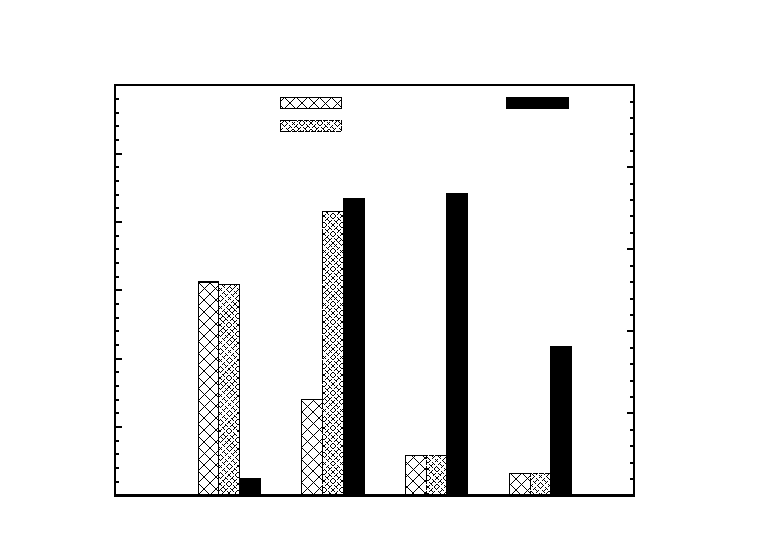
\includegraphics{conclusions-cs-en}}%
    \gplfronttext
  \end{picture}%
\endgroup
